\documentclass{article}
\usepackage[utf8x]{inputenc}
\usepackage[english,russian]{babel}
\usepackage{graphicx}
\begin{document}
\title{Применение формулы Кирхгофа для задачи миграции}
\author{\textbf{Голубев В.И.} \\ Лаборатория прикладной вычислительной геофизики МФТИ}
\maketitle
Согласно выводу (уравнени 15.208), приведённому в книге Жданова, распределение давления для
задачи акустики, показывающее также и положение отражающих границ,
может быть найдено на основе формулы Рэлея для случая горизонтальной плоскости
наблюдения:
\begin{equation}
\label{rayleigh_migration}
U^m(\vec{r'},0) = -\frac{1}{2\pi}\frac{\partial}{\partial z'}
	\int_S \frac{U(\vec{r},\frac{2|\vec{r'}-\vec{r}|}{c})}{|\vec{r'}-\vec{r}|}ds,
\end{equation}
где $U$ - скалярное поле давления, $\vec{r}$ - координата на поверхности, в которой записывается
сейсмограмма, $\vec{r'}$ - координата в объёме, где ищется мигрированное изображение, $c$ - скорость распространения возмущения, стоящая в волновом уравнении (уравнение 13.54):
\begin{equation}
\label{wave_equation}
\nabla^2P(\vec{r},t) - \frac{1}{c^2(\vec{r})}\frac{\partial^2}{\partial t^2}
	P(\vec{r},t) = - F^e(\vec{r},t).
\end{equation}

Рассмотрим простейший случай, когда расчётная сетка кубическая, и на поверхности сейсмоприёмники расположены в каждом её узле.
В таком случае формула (\ref{rayleigh_migration}) может быть записана в виде:
\begin{equation}
\label{rayleigh_migration_discrete}
U^m(i,j,k) = -\frac{1}{2\pi}\frac{\sum\limits_{l,m} \frac{U(l,m,\frac{2d(i,j,k+1,l,m)}{c})}{d(i,j,k+1,l,m)}\delta x \delta y - \sum\limits_{l,m} \frac{U(l,m,\frac{2d(i,j,k,l,m)}{c})}{d(i,j,k,l,m)}\delta x \delta y}{\delta z},
\end{equation}
где $d(i,j,k,l,m)=\sqrt{(l-i)^2(\delta x)^2 + (m-j)^2(\delta y)^2  + (k)^2(\delta z)^2}$, а начало координат находится в точке $(i,j,k)=(0,0,0)$.
В дальнейшем может быть проведено обобщение на случай произвольной (на дневной поверхности!) расстановки приёмников.

Был реализован прототип вычислителя, работающего по описанному алгоритму.
Для простоты не проводилось никакой интерполяции ни во временной области, ни в пространственной области для сейсмограмм, а просто брались значения из ближайшего пространственно-временного отсчёта.
Выполнено тестирование на двух задачах миграции.
В первом случае задавалась синтетическая сейсмограмма, полученная при отклике, инициированном продольной вертикально падающей волной с шириной фромнта 400 м, от границы раздела, расположенной на глубине 1000 м.
Во втором случае граница раздела у $\frac{1}{3}$ области по горизонтали (считая от начала координат) находилась на глубине 500 м, у $\frac{2}{3}$ - на глубине 1000 м.
Вся расчётная область составляет 1500 м.
На рис. \ref{layers_inverted} представлено изображение, полученное после процедуры миграции.
\begin{figure}[ht]
  \center
  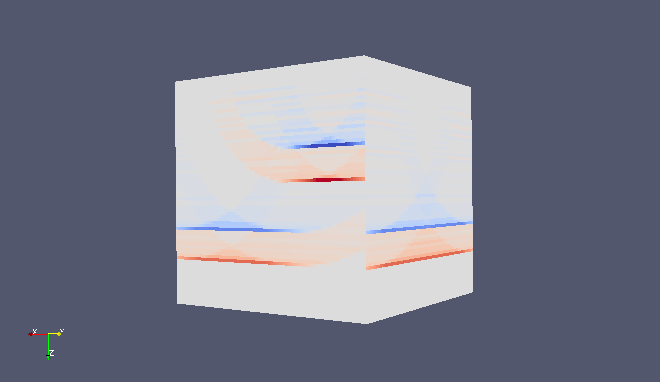
\includegraphics[scale=0.5]{pic/layers_inverted.png}
  \caption{Мигрированное изображение (слева - разрывная граница, справа - сплошная). Синий цвет - отрицательные значения, красный - положительные.}
\label{layers_inverted}
\end{figure}
\end{document}
